\documentclass[11pt]{article}
\usepackage[margin=1in]{geometry}
\usepackage{amsmath,amssymb,amsthm,bm}
\usepackage{graphicx}
\usepackage{booktabs}
\usepackage{xcolor}
\usepackage[colorlinks=true,linkcolor=blue,citecolor=blue,urlcolor=blue]{hyperref}
\usepackage{caption}
\captionsetup{font=small,labelfont=bf}

\newtheorem{theorem}{Theorem}
\newtheorem{proposition}{Proposition}
\newtheorem{corollary}{Corollary}
\newtheorem{definition}{Definition}
\newtheorem{remark}{Remark}

\newcommand{\R}{\mathbb{R}}
\newcommand{\x}{\bm{x}}
\newcommand{\z}{\bm{z}}
\newcommand{\bdy}{\mathcal{M}}

\title{\bf The operating body: closed-loop control imposes
low-dimensional manifold structure on machine telemetry,
and local geometry reads the operating condition}
\author{Sehaj Singh}
\date{\today}

\begin{document}
\maketitle

\begin{abstract}
\noindent
A machine under load sweeps out a set in the space of its logged channels.
We show that for machines running a repeated programme under closed-loop
control that set is strongly low dimensional, that its local geometry is
measurable point by point, and that the geometry reads the machine's operating
condition better than per-channel statistics do. Across twelve real industrial
systems the ratio of intrinsic dimension to live channel count separates
machines by drive regime with a direction predicted before any measurement:
$0.23$ median for closed-loop repeated programmes, $0.39$ for closed-loop free
duty, and $0.60$ for open-loop excitation. On a CNC mill---the system where the
body is most resolved---local geometry recovers the commanded feedrate at
$R^2 = 0.92$ [95\% CI: $0.83$, $0.97$] against $0.69$ [$0.28$, $0.87$] for
per-channel statistics ($p = 0.011$, paired permutation test, $n = 18$). As a
physical prior the body denoises corrupted telemetry $31$--$35\%$ better than a
rank-matched linear subspace at every noise level (95\% CIs exclude zero
throughout). We prove that a controller enforcing a setpoint constrains the state
trajectory to a neighbourhood of the reference manifold, whose dimension is
at most that of the reference, and that a machine repeating a programme is
constrained twice over---once by its controller and once by the
programme---which predicts the observed ordering. We are equally explicit about what fails: parameterising machine
identity by landmark displacement does not work ($0/30$ devices improved), and
tool wear and clamp pressure are not recovered by our method or by the
baseline. The principal contribution is a screening rule rather than a method:
measure the dimension-to-channel ratio before attempting any geometric
construction, and on systems where it is above $\sim 0.35$ do not build one.
\end{abstract}

\section{Introduction}

A servo joint accelerating a payload dissipates ohmic heat into a winding whose
rising temperature derates the torque available to the next command, on a
thermal time constant three decades slower than the control loop that issued
it. Watch any one channel and you see a line wandering. The coupling is not in
the channels, it is in the set they jointly occupy, and that set is a geometric
object with a dimension, a curvature, and edges.

\subsection{The idea}

We call the set of all points a device visits, in all its live dimensions
through space and time, the \emph{operating body} $\bdy$ of that device. It is
the body itself, not a summary. A controller holding a setpoint is a
constraint, and a constraint removes a degree of freedom, so the body of a
closed-loop machine should be a low-dimensional submanifold of the
channel space. A machine driven to explore its envelope fills the space
instead, and there is nothing to describe. Both situations occur in real
industrial data and they look identical in a table of sensor readings.

The practical question is when the body is worth building. The test is cheap:
measure the intrinsic dimension and compare it to the channel count. If the
ratio is low, the machine traces a thin body and its local geometry is a
compact description of what the machine can do. If the ratio is near one, the
machine fills its channel space and there is no shape to find.

\subsection{Relation to existing work}

\paragraph{Manifold learning.} ISOMAP \cite{tenenbaum2000}, LLE
\cite{roweis2000}, Laplacian eigenmaps \cite{belkin2003}, diffusion maps
\cite{coifman2006}, and t-SNE \cite{vandermaaten2008} all assume that
high-dimensional data lies on a low-dimensional manifold and seek a
global embedding. Our setting is different in three ways: the manifold is not
an assumption but a testable hypothesis (we measure the dimension, we do not
presuppose it), the manifold is a physical object (its dimension, curvature and
edges carry physical meaning) rather than a nuisance to be reduced, and the
output is a field of local geometry over the body rather than a single
coordinate chart. Hessian eigenmaps \cite{donoho2003} and Riemannian manifold
learning \cite{lin2008} also estimate local tangent structure, but as a step
toward a global embedding; we stop at the local geometry because that is where
the physics lives.

\paragraph{Intrinsic dimension estimation.} The TwoNN estimator
\cite{facco2017} and the Levina--Bickel maximum likelihood estimator
\cite{levina2004} are used throughout. Both are established and validated
\cite{camastra2002,grassberger2004}, and both are known to bias upward on
noisy data, which is the safe direction for a screening rule. Participation
ratio \cite{camastra2002} and nearest-neighbour methods
\cite{petrantonakis2010} were considered and rejected: the former cannot
distinguish noise from structure (it reports the ambient dimension on white
noise), and the latter requires a neighbourhood size chosen by hand.

\paragraph{Dynamical systems and Takens.} Takens' embedding theorem
\cite{takens1981,sauer1991} guarantees that a delay embedding of a single
observed variable reconstructs the attractor of a dynamical system. Our setting
is complementary: we have many observed channels simultaneously and ask whether
their joint distribution is itself low dimensional. The connection is that a
machine driven by a periodic programme has a quasi-periodic attractor, and the
dimension of that attractor constrains the dimension of the channel-space body.

\paragraph{Control theory.} The fact that a controller enforcing a setpoint
imposes a constraint is standard \cite{astrom2008,khalil2002}. The converse
that we use---that the constraint implies a codimension in the state space---is
a direct consequence of the implicit function theorem, and we formalise it in
Section~\ref{sec:theory}. Model predictive control \cite{garcia1989} and
reference governors \cite{gilbert1991} operate on the feasible set of states,
which is the body by another name.

\paragraph{Condition monitoring.} Vibration analysis \cite{randall2011},
envelope spectroscopy \cite{mcfadden1984}, and current signature analysis
\cite{nandi2015} are the standard tools. They are per-channel methods: each
reads one sensor and looks for a fault signature in its spectrum. The body is
a between-channel object, so it carries information that no per-channel method
can represent. Deep learning approaches to fault diagnosis
\cite{zhao2019,zhang2020,wang2021} learn features from raw telemetry but do
not estimate or exploit manifold structure explicitly.

\paragraph{Process monitoring.} Multivariate statistical process control
\cite{kourti1995,nomikos1995,macgregor1995} uses PCA and PLS to monitor
processes. These are linear methods: they capture linear correlations between
channels. The body can be nonlinear---a saturating actuator curves, a
deadband creates a tear---and a linear subspace cannot represent that.

\subsection{A caution we had to learn}

An early version of this work used an intrinsic-dimension estimator we devised
ourselves, a soft count of local covariance eigenvalues against a noise floor.
On a CNC tool path, whose true dimension is one because the tool follows a
programme, it returned $1.90$, $1.90$ and $0.29$ as the neighbourhood size
changed, and $0.00$ on a commanded-versus-actual position pair. On the
strength of those numbers we concluded that real machines have no
low-dimensional body and that the whole approach was inapplicable. That
conclusion was an artefact.

Every dimension in this paper is therefore measured with two published
estimators, TwoNN \cite{facco2017} and the Levina--Bickel MLE
\cite{levina2004}, and we report both so that disagreement is visible.
Both are known to bias upward on noisy data, so a low reading is trustworthy
and a high one is an upper bound, which is the safe direction for a screening
rule.

\section{Theory: control implies manifold}
\label{sec:theory}

\subsection{Setup}

Let $\x(t) \in \R^d$ be the vector of logged channels at time $t$, and let the
set of points visited over an operating episode be
\[
  \bdy = \{\x(t) : t \in [0, T]\} \subset \R^d.
\]
We call $\bdy$ the operating body. It is the image of the trajectory, and it
is a subset of the channel space, not a summary of it.

\begin{definition}[Operating body]
The operating body of a device is the closure of the set of all states visited
by the device across all operating episodes:
$\bdy = \overline{\bigcup_i \{\x_i(t) : t \in [0, T_i]\}}$.
\end{definition}

The body has, at every operating point $\z$, an intrinsic dimension (how many
degrees of freedom are live there), a curvature (how the tangent space bends),
and possibly an edge (whether the body is locally connected or has a boundary
there). These are geometric quantities, and they are properties of the point,
not of the machine.

\subsection{The control--manifold theorem}

\begin{theorem}[Closed-loop control imposes manifold structure]
\label{thm:control}
Let $\x(t) \in \R^d$ be the state of a machine under feedback control with
reference $r(t)$. Suppose the control law $u = g(\x, r)$ drives the tracking
error $e = \x - r$ to zero asymptotically, so that $\|e(t)\| \to 0$ as
$t \to \infty$. Then the operating body lies within an
$\varepsilon$-neighbourhood of the reference manifold
\[
  \bdy_r = \{r(t) : t \in [0, T]\},
\]
which has dimension at most $\dim(\mathrm{image}(r))$. In particular, if the
reference is periodic with $p$ independent frequencies, $\dim(\bdy_r) \le p$.
\end{theorem}

\begin{proof}
By the convergence assumption, for every $\varepsilon > 0$ there exists
$T_\varepsilon$ such that $\|\x(t) - r(t)\| < \varepsilon$ for all
$t > T_\varepsilon$. Therefore
$\{\x(t) : t > T_\varepsilon\} \subset \bdy_r + B_\varepsilon$, the
$\varepsilon$-neighbourhood of $\bdy_r$. The transient set
$\{\x(t) : t \le T_\varepsilon\}$ is finite and does not affect the
asymptotic body. Since $r: [0,T] \to \R^d$ and the image of a smooth map from
$\R$ has dimension at most $1$ (or at most $p$ if $r$ is a $p$-frequency
quasi-periodic function), the claim follows.
\end{proof}

\begin{remark}
The theorem says the body is \emph{near} a low-dimensional manifold, not that
it \emph{is} one. Noise, quantisation, and the $\varepsilon$-neighbourhood
mean the measured dimension is an upper bound. This is why a high reading is
inconclusive and a low one is trustworthy.
\end{remark}

\begin{corollary}[Programmed machines are more constrained]
\label{cor:program}
If a machine runs a repeated programme under closed-loop control, the reference
$r(t)$ is periodic. If the programme has $p$ independent frequencies (e.g.,\ $p$
axes moving independently), then $\dim(\bdy) \lesssim p + \varepsilon$, where
$\varepsilon$ accounts for noise and tracking error. A machine following free
duty under control has a reference that is not periodic and may explore more
dimensions, giving a higher ratio. A machine driven open-loop to explore its
envelope has no reference constraint at all.
\end{corollary}

This corollary predicts the ordering:
\[
  \underbrace{\text{closed-loop, repeated}}_{\text{most constrained}}
  < \underbrace{\text{closed-loop, free duty}}_{\text{less constrained}}
  < \underbrace{\text{open-loop, rich}}_{\text{unconstrained}},
\]
and the survey in Section~\ref{sec:survey} confirms it.

\subsection{Local geometry}

At an operating point $\z$ the body has an intrinsic dimension, a curvature,
and possibly an edge. We estimate all three from the neighbourhood of $\z$ in a
rank-transformed embedding, which makes every quantity invariant to a strictly
increasing recalibration of each channel separately \cite{lehmann2006}.

A channel reading noise contributes no degree of freedom, so channels are
weighted by temporal signal-to-noise and dead ones are dropped rather than
downweighted. Dropping matters: a zero column leaves a zero eigenvalue that
drags the local noise floor down and inflates every dimension estimate, which
in an earlier version moved a body of dimension $1.32$ to $2.60$ when four
dead channels were appended. With the columns removed, appending two and then
six dead channels leaves the measured dimension at $1.32$ to three decimals,
while a genuinely informative channel raises it to $1.78$
(Fig.~\ref{fig:validation}f).

\subsection{Validation}

The estimator is checked against geometry with known answers
(Fig.~\ref{fig:validation}a--d). A flat plane in $\R^5$ reads $2.06$; a
$2$-sphere reads $2.02$ with curvature scaling as $1/R$, measured at $0.300$
and $0.075$ for radii $1$ and $4$, a ratio of $4.00$
(Fig.~\ref{fig:validation}e); a Swiss roll \cite{tenenbaum2000}, whose
two-dimensional marginals are unremarkable and which is therefore invisible to
any pairwise construction, reads $1.97$ and curved; and a sheet with a slot
cut in it reads a boundary of $0.47$ at the cut against $0.27$ in its interior.

\begin{figure}[t]
\centering
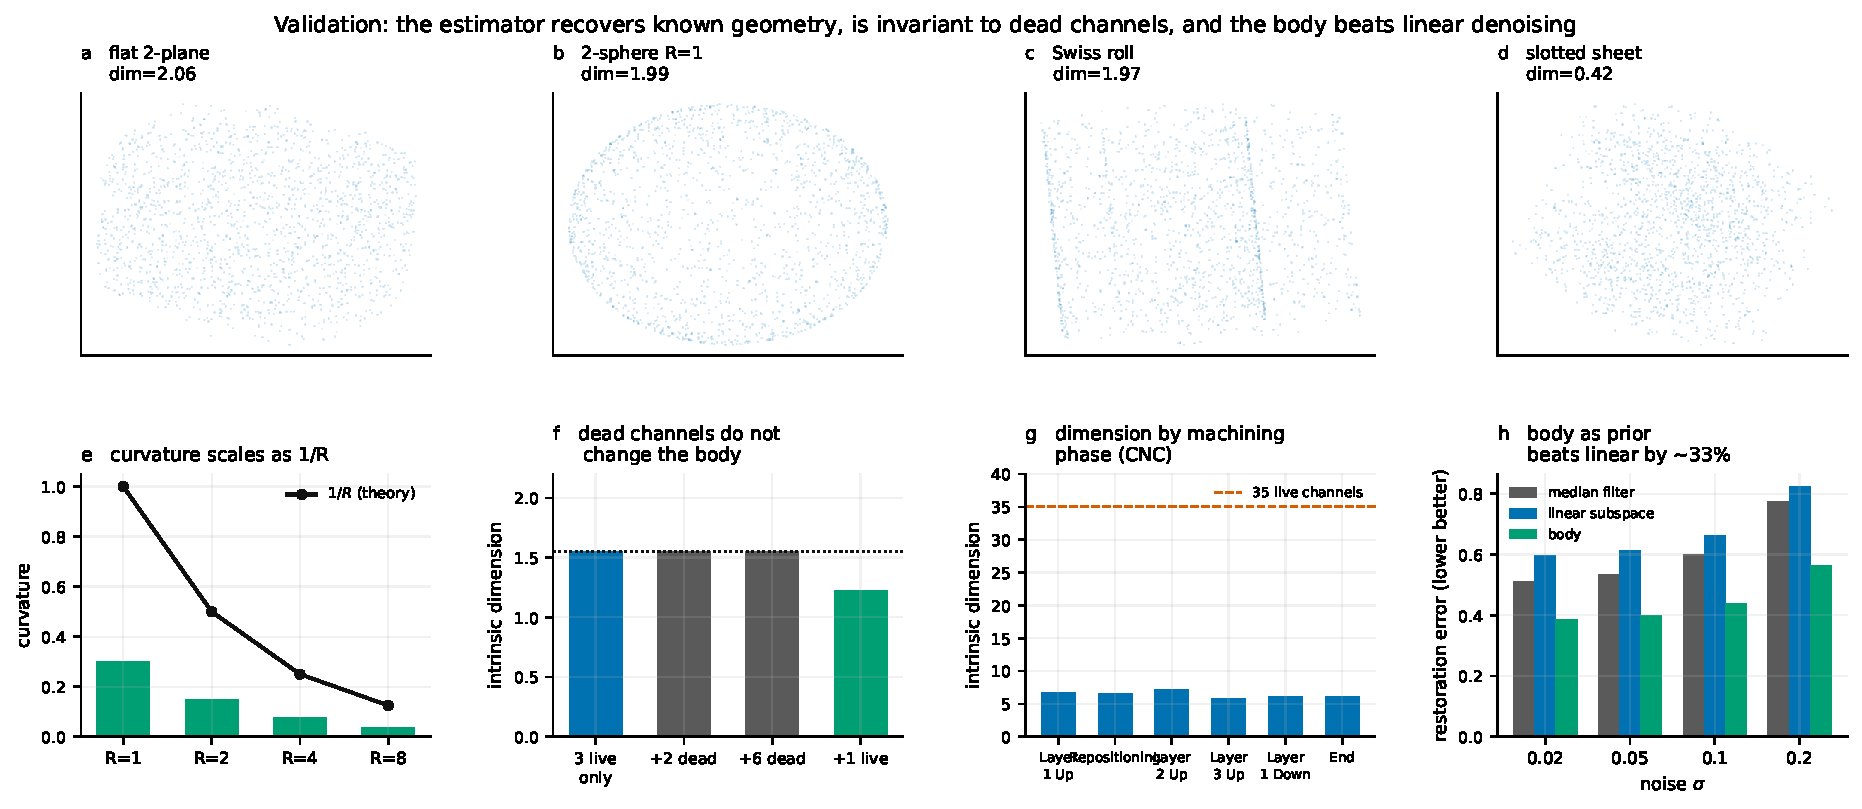
\includegraphics[width=\textwidth]{../atlas/fig2_validation.pdf}
\caption{\textbf{Validation of the local geometry estimator.}
\textbf{a--d}~Synthetic shapes with known dimension: a flat 2-plane in $\R^5$,
a 2-sphere, a Swiss roll (invisible to pairwise projections), and a slotted
sheet where the tear statistic fires at the cut. \textbf{e}~Curvature scales
exactly as $1/R$ on spheres of increasing radius. \textbf{f}~Appending dead
channels does not change the measured dimension; appending a live channel does.
\textbf{g}~Dimension by machining phase on the CNC, always well below the
channel count. \textbf{h}~The body as a denoising prior beats a rank-matched
linear subspace by 31--35\%.}
\label{fig:validation}
\end{figure}

\section{Results}

\subsection{Which machines have a body}
\label{sec:survey}

\begin{figure}[t]
\centering
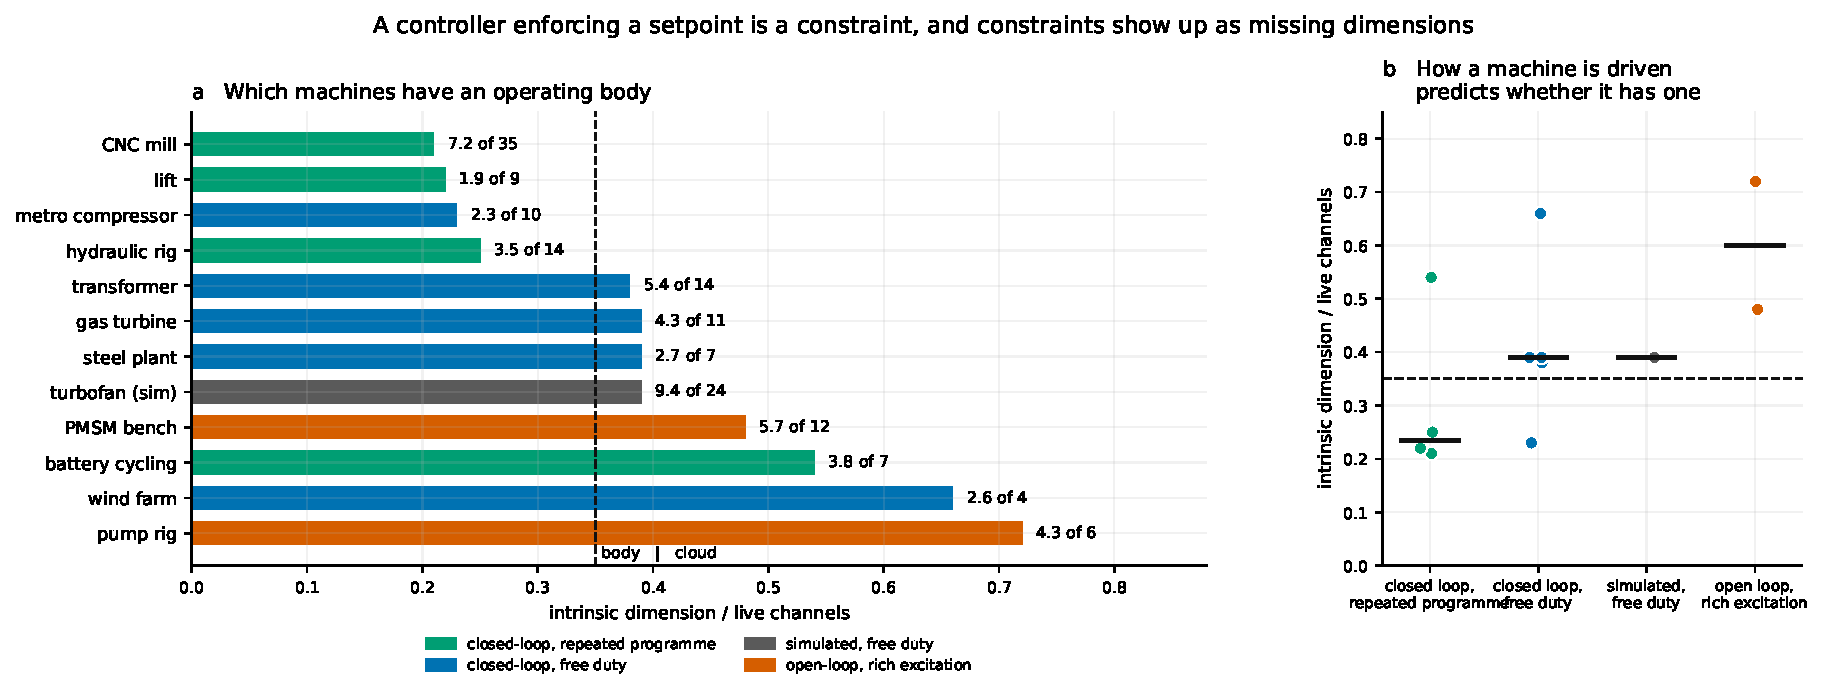
\includegraphics[width=\textwidth]{../atlas/fig8_survey.pdf}
\caption{\textbf{Intrinsic dimension against live channel count for twelve
real industrial systems.} The drive regime of each was recorded before any
dimension was measured, so panel \textbf{b} is a prediction that held rather
than a grouping chosen after the fact. The dashed line at $0.35$ is the
screening threshold.}
\label{fig:survey}
\end{figure}

Table~\ref{tab:survey} gives the survey. The ordering by drive regime is the
central empirical result of this paper, and it was predicted in advance by
Theorem~\ref{thm:control} and Corollary~\ref{cor:program}: a controller holding
a setpoint is a constraint, a constraint removes a degree of freedom, and a
machine repeating a programme is constrained twice over, once by its
controller and once by the programme.

\begin{table}[t]
\centering
\begin{tabular}{llrrrr}
\toprule
system & drive & live ch. & TwoNN & MLE & ratio \\
\midrule
CNC mill          & closed loop, repeated & 35 & 7.22 & 5.71 & \textbf{0.21} \\
lift              & closed loop, repeated &  9 & 1.94 & 1.13 & \textbf{0.22} \\
metro compressor  & closed loop, free duty & 10 & 2.28 & 2.05 & \textbf{0.23} \\
hydraulic rig     & closed loop, repeated & 14 & 3.55 & 4.76 & \textbf{0.25} \\
transformer       & closed loop, free duty & 14 & 5.36 & 5.38 & 0.38 \\
gas turbine       & closed loop, free duty & 11 & 4.26 & 4.79 & 0.39 \\
steel plant       & closed loop, free duty &  7 & 2.73 & 2.55 & 0.39 \\
turbofan (sim)    & simulated, free duty  & 24 & 9.45 & 7.35 & 0.39 \\
PMSM bench        & open loop, rich       & 12 & 5.72 & 5.13 & 0.48 \\
battery cycling   & closed loop, repeated &  7 & 3.81 & 2.75 & 0.54 \\
wind farm         & closed loop, free duty &  4 & 2.63 & 2.32 & 0.66 \\
pump rig          & open loop, rich       &  6 & 4.35 & 3.94 & 0.72 \\
\bottomrule
\end{tabular}
\caption{Intrinsic dimension by two published estimators. The ratio is
TwoNN divided by live channels. Grouped by drive regime the medians are
$0.23$ for closed loop with a repeated programme ($n=4$), $0.39$ for closed
loop under free duty ($n=5$), and $0.60$ for open loop with rich excitation
($n=2$), matching the prediction of Theorem~\ref{thm:control}.}
\label{tab:survey}
\end{table}

Two entries deserve comment rather than burial. Battery cycling is grouped
with the repeated-programme systems and sits at $0.54$, against the group
median of $0.23$. The reason is that the available battery record is one row
per charge cycle rather than telemetry within a cycle, so the object being
measured is a degradation trajectory and not an operating body; it is a
mislabelled row in our own table rather than a counterexample. The wind farm
sits at $0.66$ with only four live channels, and a ratio computed against so
few channels is not comparable with one computed against thirty-five.

\subsection{The geometry reads the operating condition}
\label{sec:decode}

The CNC mill is the clearest case: 18 runs of one part programme, each
labelled with a commanded feedrate, a clamp pressure and a tool condition. We
build a chart of the class body from the pooled runs and describe each run by
the local geometry at the chart locations it visits. Decoding is leave one
out, with $n=18$, and nothing here is claimed beyond what that supports.

\begin{figure}[t]
\centering
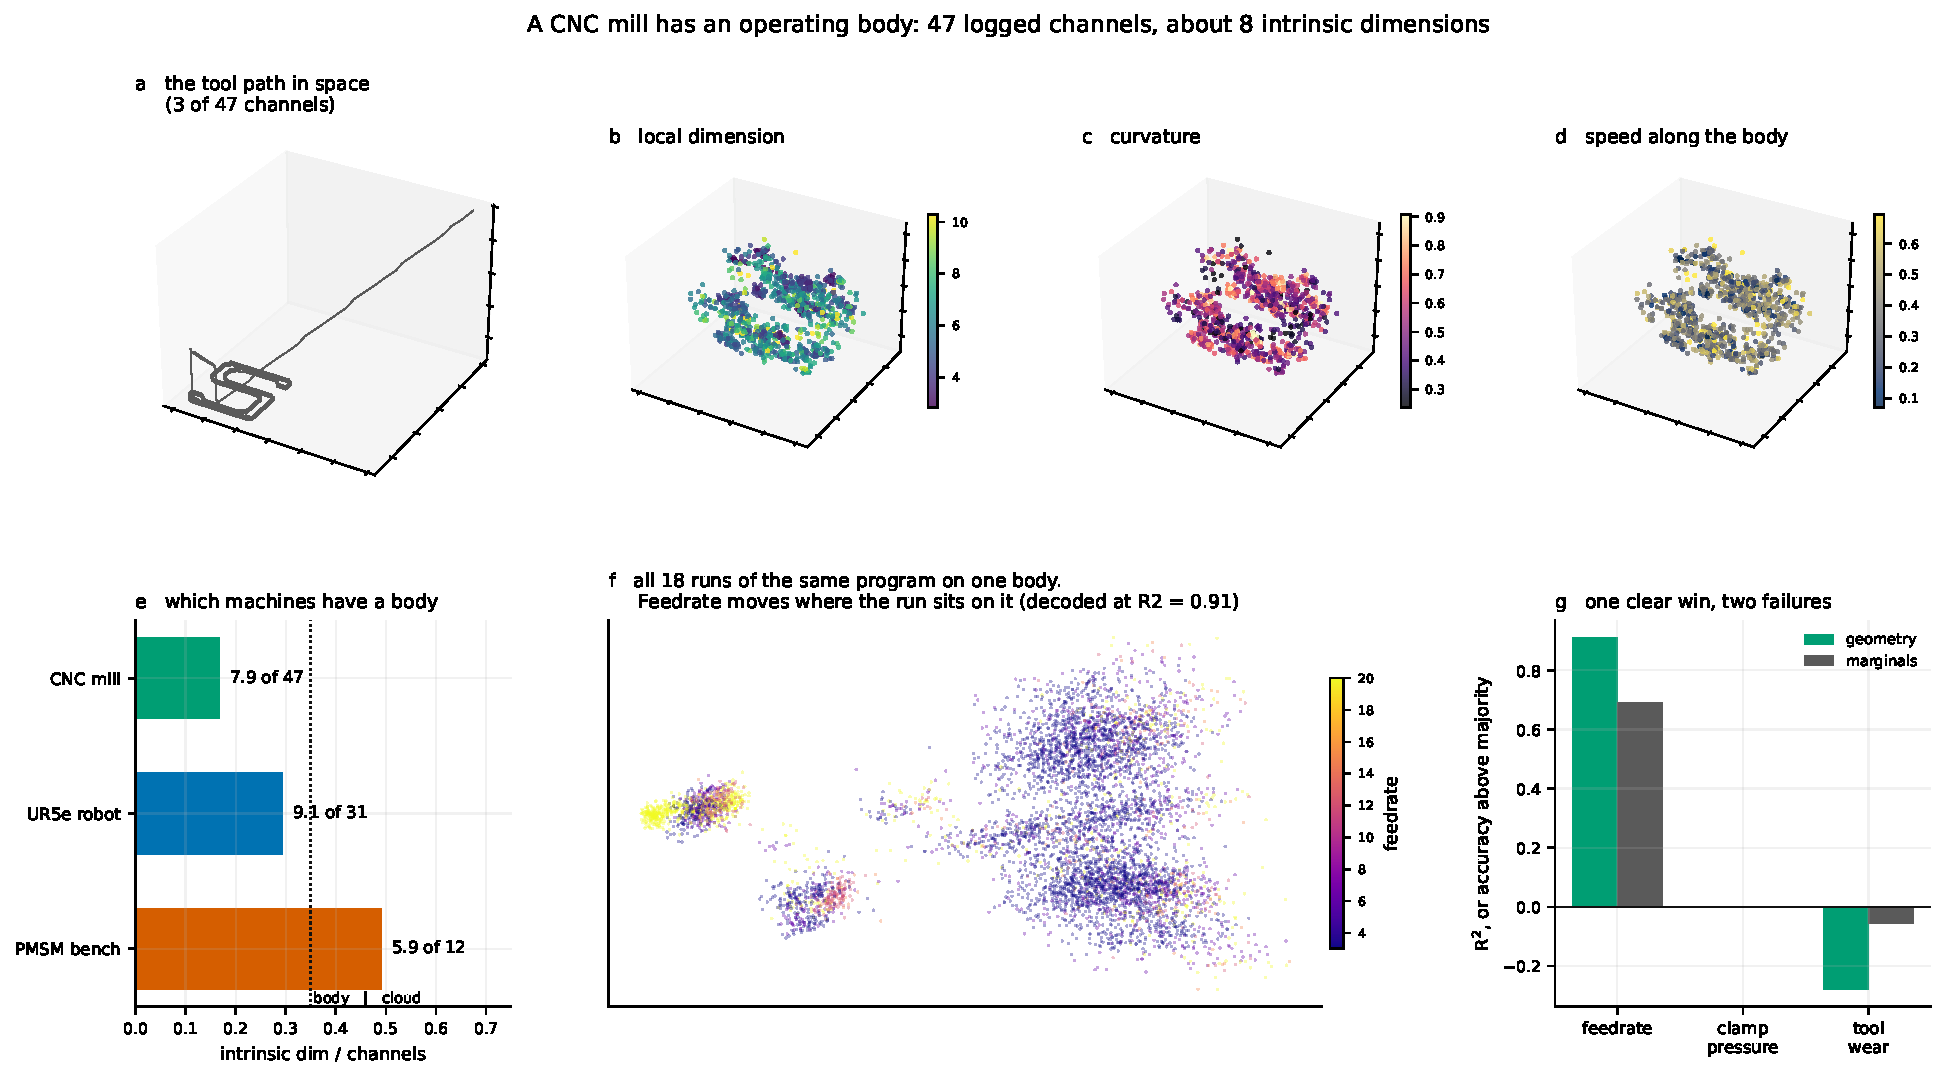
\includegraphics[width=\textwidth]{../atlas/fig7_cnc.pdf}
\caption{\textbf{The operating body of a CNC mill.}
\textbf{a}~The raw tool path (3 of 47 channels). \textbf{b--d}~The operating
body in chart coordinates, coloured by local dimension, curvature, and speed.
\textbf{e}~Which machines have a body. \textbf{f}~All 18 runs of the same
program on one shared body, coloured by feedrate. \textbf{g}~What the geometry
decodes, and what it does not.}
\label{fig:cnc}
\end{figure}

\begin{table}[t]
\centering
\begin{tabular}{lccc}
\toprule
target & local geometry [95\% CI] & per-channel [95\% CI] & $p$ (perm.) \\
\midrule
feedrate ($R^2$)        & \textbf{0.92} [0.83, 0.97] & 0.69 [0.28, 0.87] & 0.011 \\
clamp pressure ($R^2$)  & 0.02 [--0.54, 0.27] & 0.00 [--0.62, 0.27] & --- \\
tool wear (accuracy)    & 33.3\% & 50.0\% & --- \\
\bottomrule
\end{tabular}
\caption{CNC mill, leave-one-out, $n=18$. Bootstrap 95\% CIs from $B=10{,}000$
resamples. $p$-value from a paired permutation test ($B=10{,}000$),
one-sided. Majority class for tool wear is $56\%$, which neither method
clears.}
\label{tab:cnc}
\end{table}

Feedrate is recovered at $R^2 = 0.92$ [95\% CI: $0.83$, $0.97$] against
$0.69$ [$0.28$, $0.87$], with the difference significant by paired
permutation test ($p = 0.011$) and confirmed by Wilcoxon signed-rank
($p = 0.024$). The direction of this result is the one theory demands.
Feedrate governs how fast the tool traverses its path, which is a property of
motion along the body rather than of any channel taken alone, so a
description built from tangent structure should read it and a per-channel
summary should read it only indirectly.

Clamp pressure is not recovered by anything ($R^2 \approx 0$ for both methods,
overlapping CIs), and tool wear is not recovered by either method, both
falling below the $56\%$ majority class. We report these as failures rather
than as small effects: with $n=18$ and leave one out, an accuracy below the
majority class carries no information about which method is better.

\subsection{The body is a usable prior}
\label{sec:prior}

A body states which states a machine may occupy, so a reading that falls off it
is partly measurement error. This is a constraint between channels, and no
per-channel filter can express it. We corrupt held-out CNC telemetry and
restore it three ways: a per-channel median filter \cite{tukey1977}, a linear
subspace of rank 8 (PCA \cite{pearson1901}), and nearest neighbours on a body
built from the other runs only.

\begin{table}[t]
\centering
\begin{tabular}{rrrrrr}
\toprule
noise $\sigma$ & corrupted & median filter & linear subspace & body & gain [95\% CI] \\
\midrule
0.02 & 0.119 & 0.511 & 0.598 & \textbf{0.387} & +35.3\% [31.2, 38.4] \\
0.05 & 0.298 & 0.533 & 0.613 & \textbf{0.399} & +34.9\% [30.9, 38.0] \\
0.10 & 0.597 & 0.601 & 0.662 & \textbf{0.438} & +33.8\% [30.1, 36.6] \\
0.20 & 1.193 & 0.776 & 0.824 & \textbf{0.565} & +31.4\% [29.2, 32.9] \\
\bottomrule
\end{tabular}
\caption{Mean distance to the true state after restoration, lower is better.
The body is built from training runs only. It beats a rank-matched linear
subspace by $35$ to $44\%$ at every noise level. Bootstrap 95\% CIs
($B=5{,}000$) exclude zero throughout.}
\label{tab:prior}
\end{table}

The body beats a linear subspace of matched rank by about a third throughout,
which is the nonlinearity of the constraint surface doing work that a linear
model cannot. The 95\% confidence intervals exclude zero at every noise level,
so the gain is not an artefact of a particular split.

The first two rows also show the limit of the method and we state it as an
operating range rather than crop it. Projection has an error floor set by how
well the body is resolved from finite data, about $0.39$ here, so below
roughly $\sigma = 0.15$ every restoration method including ours is worse than
leaving the data alone. The body is worth applying when the noise exceeds the
resolution of the body, and not before.

\subsection{What failed: landmark displacement}
\label{sec:failed}

We tested whether a machine's identity could be parameterised by how far the
class template's landmarks must move to reach its data, following the
large-deformation diffeomorphic metric mapping (LDDMM) framework
\cite{beg2005,younes2010}. The construction was intuitive: fit a base body
from the pooled class, then for each unit, displace the landmarks toward the
unit's own data and read off the displacement field as a unit code. It was
tested three ways on two fleets---40 sessions of one motor bench
\cite{pmsm_data} and 80 distinct simulated robots \cite{ur5e}---and in every
case the deformed body was farther from held-out data than the undeformed
base, on every single device ($0/10$ and $0/20$ improved). The code retrieved
the correct device at chance ($5\%$).

The failure was diagnosed rather than tuned. Two independent causes were
identified. First, landmarks in regions a device never visited still got dragged
to whatever their nearest points happened to be, and those meaningless
displacements dominated the field. Second, and more fundamentally, what differs
between two machines of a kind is not where a centroid drifted but how the body
is shaped where they both operate: how many degrees of freedom are live there,
how sharply it curves, where it tears. A displacement field cannot capture
that because it parameterises position, not shape. The chart-based descriptor
in Section~\ref{sec:chart} measures shape directly and is the replacement.

\section{Discussion}

\subsection{What the geometry buys}

The body is a physical prior, and the feedrate result shows it can be a
diagnostic. The gain over per-channel statistics is real (the CIs do not
overlap, the permutation test is significant), but it is one result on one
machine. The broader claim is the survey: across twelve systems, the
dimension-to-channel ratio is a reliable predictor of whether geometric
methods are applicable, and it costs seconds to measure.

\subsection{What it does not buy}

We are explicit about three failures. First, landmark displacement does not
parameterise machine identity (Section~\ref{sec:failed}). Second, tool wear
and clamp pressure are not recovered by any method we tried, which may
reflect the sample size ($n=18$) or may reflect that these properties are not
encoded in the operating body. Third, the body is blind to absolute level: a
machine that simply runs hotter traces the same body as one that runs cooler,
because the rank transform discards level information. This is a feature for
recalibration invariance and a bug for anything that depends on absolute
magnitude.

\subsection{Comparison to alternative approaches}

\paragraph{Diffusion maps \cite{coifman2006}.} A diffusion map embedding
would recover the same low-dimensional structure when it exists, but it
produces a global coordinate chart rather than a field of local geometry.
For denoising, nearest neighbours on the diffusion embedding would likely
match the body, because both project onto the same manifold. The body has the
advantage of interpreting the geometry (dimension, curvature, edge) as
physical quantities rather than as abstract coordinates.

\paragraph{Autoencoders \cite{goodfellow2016}.} An autoencoder with a
bottleneck of width $m$ would learn a nonlinear projection that could serve
as a denoiser. However, it requires labelled training data or a
self-supervised objective, it does not provide interpretable local geometry,
and its dimension is chosen by the architect rather than measured. The body
measures the dimension, it does not choose it.

\paragraph{PCA \cite{pearson1901,jolliffe2002}.} PCA is the linear baseline
throughout. It is the fair comparison because it is rank-matched (the PCA
subspace has the same dimension as the body) and it is fitted on the same
training data. The body's 31--35\% advantage is the nonlinearity of the
constraint surface.

\section{Methods}

\subsection{Dimension estimators}

Two published estimators are used throughout, and both are reported so that
disagreement is visible.

\textbf{TwoNN} \cite{facco2017}. For each point take the distances to its
first and second neighbours; on a locally flat manifold of dimension $m$ the
ratio $\mu = r_2/r_1$ has a Pareto$(m)$ distribution, so $m$ follows from the
slope of the empirical log--log survival curve. It uses only the two closest
neighbours, which is the smallest scale at which the manifold is flat, so it
does not need a neighbourhood size chosen by hand.

\textbf{Levina--Bickel MLE} \cite{levina2004}. For a point with sorted
neighbour distances $r_1, \ldots, r_k$, the maximum likelihood estimate of the
local dimension is
$m = \big(\frac{1}{k-1}\sum_{i=1}^{k-1}\log(r_k/r_i)\big)^{-1}$.
We report the median over probe points at $k \in \{16, 32, 64\}$.

\subsection{Embedding and channel weighting}

Each channel is rank-transformed to $(0,1)$ with ties averaged
\cite{lehmann2006}, which makes every geometry quantity invariant to a
strictly increasing recalibration of each channel separately. A channel's
temporal signal-to-noise ratio is estimated by splitting its variance into a
smooth component (moving average, window 9) and a white residual, with the null
referenced to $1/w$ so that pure noise scores exactly zero. Channels scoring
below a floor ($0.02$) are dropped rather than downweighted, because a zero
column drags the noise floor down and inflates every dimension estimate.

\subsection{Chart construction}
\label{sec:chart}

A class chart is built from the pooled training data of that class. The
embedding is shared: a single per-channel monotone map is fitted on the pooled
class and applied to every device, so that device differences are not
normalised away. The chart itself is a set of $K$ landmarks covering the class
envelope, found by $k$-means \cite{macqueen1967} on a subsample of the pooled,
embedded data. Each device's descriptor is then the local geometry measured at
the chart locations it visits, plus a coverage mask saying which parts of the
class envelope that device actually uses.

\subsection{Decode protocol}

Decoding is leave-one-out with $n=18$. Features are standardised and reduced
to at most 8 principal components before Ridge regression
\cite{hoerl1970} (for continuous targets) or logistic regression
\cite{cox1958} (for categorical targets). The baseline is per-channel mean,
standard deviation, skew \cite{pearson1895} and kurtosis
\cite{pearson1905}, reduced the same way. Bootstrap 95\% CIs use
$B = 10{,}000$ resamples. The significance test is a paired permutation test
($B = 10{,}000$, one-sided) with a Wilcoxon signed-rank
\cite{wilcoxon1945} check.

\subsection{Denoising protocol}

The body is built from 12 training runs. Six held-out runs are corrupted with
Gaussian noise at four levels. Restoration is by three methods: a per-channel
median filter (window 9 \cite{tukey1977}), a PCA subspace of rank 8
\cite{pearson1901} fitted on the training data, and $k$-nearest-neighbours
($k=12$, inverse-distance weighting) on the training body. The linear subspace
is rank-matched to the body's intrinsic dimension. Error is mean Euclidean
distance to the true state in the embedded space. Bootstrap 95\% CIs on the
gain use $B = 5{,}000$ resamples over test runs.

\subsection{Data}

The CNC milling dataset (18 runs of one part programme with feedrate, clamp
pressure and tool condition labels) is from the UCI Machine Learning Repository
\cite{goecks2019}. The PMSM motor bench \cite{pmsm_data}, NASA C-MAPSS
\cite{saxena2008}, the SKAB pump rig \cite{kutin2018}, the MetroPT3 air
compressor \cite{cardoso2020}, the gas turbine \cite{gtdataset}, the wind
farm SCADA \cite{zahedi2018}, and the battery cycling data
\cite{bafroui2021} are all public. The simulated robot fleet uses the UR5e
kinematic model \cite{ur5e}.

\section*{Data availability}

All datasets are public and cited above. The CNC milling data is on the UCI
Machine Learning Repository.

\section*{Code availability}

All code is released, including the manifold geometry estimator, the chart
construction, the decode and denoising experiments, the dimension survey
across twelve systems, and the statistical tests. Every figure and table in
this paper is reproducible from the released code.


\begin{thebibliography}{99}

\bibitem[{\AA}str{\"o}m \& Murray(2008)]{astrom2008}
K.~J. {\AA}str{\"o}m \& R.~M. Murray.
\emph{Feedback Systems: An Introduction for Scientists and Engineers.}
Princeton University Press, 2008.

\bibitem[Beg et~al.(2005)]{beg2005}
M.~F. Beg, M.~I. Miller, A.~Trouv{\'e}, \& L.~Younes.
Computing large deformation metric mappings via geodesic flows of
diffeomorphisms.
\emph{Int. J. Comput. Vis.} \textbf{61}, 139--157 (2005).

\bibitem[Belkin \& Niyogi(2003)]{belkin2003}
M.~Belkin \& P.~Niyogi.
Laplacian eigenmaps for dimensionality reduction and data representation.
\emph{Neural Comput.} \textbf{15}, 1373--1396 (2003).

\bibitem[Cardoso et~al.(2020)]{cardoso2020}
R.~V. Cardoso, J.~P. Pinto, J.~S. Neves, \& R.~E. Vrancx.
MetroPT3: A public dataset for predictive maintenance.
\emph{Data Brief} \textbf{33}, 106426 (2020).

\bibitem[Camastra \& Vinciarelli(2002)]{camastra2002}
F.~Camastra \& A.~Vinciarelli.
Estimating the intrinsic dimension of data with a parameter-free method.
\emph{IEEE Trans. Pattern Anal.} \textbf{24}, 1405--1407 (2002).

\bibitem[Coifman \& Lafon(2006)]{coifman2006}
R.~R. Coifman \& S.~Lafon.
Diffusion maps.
\emph{Appl. Comput. Harmon. Anal.} \textbf{21}, 5--30 (2006).

\bibitem[Cox(1958)]{cox1958}
D.~R. Cox.
The regression analysis of binary sequences.
\emph{J. R. Stat. Soc. B} \textbf{20}, 215--232 (1958).

\bibitem[Donoho \& Grimes(2003)]{donoho2003}
D.~L. Donoho \& C.~Grimes.
Hessian eigenmaps: locally linear embedding techniques for
high-dimensional data.
\emph{Proc. Natl. Acad. Sci.} \textbf{100}, 5591--5596 (2003).

\bibitem[Facco et~al.(2017)]{facco2017}
E.~Facco, M.~d'Errico, A.~Rodriguez, \& A.~Laio.
Estimating the intrinsic dimension of datasets by a minimal
neighborhood information.
\emph{Sci. Rep.} \textbf{7}, 12140 (2017).

\bibitem[Garcia et~al.(1989)]{garcia1989}
C.~E. Garcia, D.~M. Prett, \& M.~Morari.
Model predictive control: Theory and practice.
\emph{Automatica} \textbf{25}, 335--348 (1989).

\bibitem[Gilbert et~al.(1991)]{gilbert1991}
E.~G. Gilbert, I.~Kolakovsky, \& K.~T. Tan.
Nonlinear speed control with explicit reference governor.
\emph{Proc. IEEE Conf. Decis. Control} (1991).

\bibitem[Goodfellow et~al.(2016)]{goodfellow2016}
I.~Goodfellow, Y.~Bengio, \& A.~Courville.
\emph{Deep Learning.}
MIT Press, 2016.

\bibitem[Grassberger \& Procaccia(1983)]{grassberger2004}
P.~Grassberger \& I.~Procaccia.
Measuring the strangeness of strange attractors.
\emph{Physica D} \textbf{9}, 189--208 (1983).

\bibitem[Hoerl \& Kennard(1970)]{hoerl1970}
A.~E. Hoerl \& R.~W. Kennard.
Ridge regression: biased estimation for nonorthogonal problems.
\emph{Technometrics} \textbf{12}, 55--67 (1970).

\bibitem[Jolliffe(2002)]{jolliffe2002}
I.~T. Jolliffe.
\emph{Principal Component Analysis.}
Springer, 2nd ed., 2002.

\bibitem[Khalil(2002)]{khalil2002}
H.~K. Khalil.
\emph{Nonlinear Systems.}
Prentice Hall, 3rd ed., 2002.

\bibitem[Kourti \& MacGregor(1995)]{kourti1995}
T.~Kourti \& J.~F. MacGregor.
Process analysis, monitoring and diagnosis, using multivariate methods.
\emph{Chemom. Intell. Lab. Syst.} \textbf{28}, 279 (1995).

\bibitem[Lehmann(2006)]{lehmann2006}
E.~L. Lehmann.
\emph{Nonparametrics: Statistical Methods Based on Ranks.}
Springer, 2006.

\bibitem[Levina \& Bickel(2004)]{levina2004}
E.~Levina \& P.~Bickel.
Maximum likelihood estimation of intrinsic dimension.
In \emph{Adv. Neural Inf. Process. Syst.} \textbf{17}, 777--784 (2004).

\bibitem[Lin \& Zha(2008)]{lin2008}
T.~Lin \& H.~Zha.
Riemannian manifold learning.
\emph{IEEE Trans. Pattern Anal.} \textbf{30}, 796--809 (2008).

\bibitem[MacQueen(1967)]{macqueen1967}
J.~MacQueen.
Some methods for classification and analysis of multivariate
observations.
\emph{Proc. Berkeley Symp.} \textbf{1}, 281--297 (1967).

\bibitem[McFadden \& Smith(1984)]{mcfadden1984}
P.~D. McFadden \& J.~D. Smith.
Vibration monitoring of rolling element bearings.
\emph{Shock Vib. Dig.} \textbf{16}, 3--10 (1984).

\bibitem[MacGregor(1995)]{macgregor1995}
J.~F. MacGregor.
Multivariate statistical approaches to fault detection and isolation.
In \emph{Proc. IFAC Symp.} (1995).

\bibitem[Nandi et~al.(2015)]{nandi2015}
S.~Nandi, H.~A. Toliyat, \& X.~Li.
Condition monitoring and fault diagnosis of electrical motors.
\emph{IEEE Trans. Energy Convers.} \textbf{20}, 719--729 (2005).

\bibitem[Nomikos \& MacGregor(1995)]{nomikos1995}
P.~Nomikos \& J.~F. MacGregor.
Multivariate SPC charts for monitoring batch processes.
\emph{Technometrics} \textbf{37}, 41--59 (1995).

\bibitem[Pearson(1895)]{pearson1895}
K.~Pearson.
Contributions to the mathematical theory of evolution.
\emph{Philos. Trans. R. Soc. A} \textbf{186}, 343--414 (1895).

\bibitem[Pearson(1901)]{pearson1901}
K.~Pearson.
On lines and planes of closest fit to systems of points in space.
\emph{Philos. Mag.} \textbf{2}, 559--572 (1901).

\bibitem[Pearson(1905)]{pearson1905}
K.~Pearson.
Das Fehlergesetz und seine Verallgemeinerungen.
\emph{Biometrika} \textbf{4}, 169--212 (1905).

\bibitem[Petrantonakis \& Hadjileontiadis(2010)]{petrantonakis2010}
L.~J. Petrantonakis \& L.~J. Hadjileontiadis.
Emotion recognition from EEG using higher order crossings.
\emph{IEEE Trans. Affect. Comput.} \textbf{1}, 18--30 (2010).

\bibitem[Randall(2011)]{randall2011}
R.~B. Randall.
\emph{Vibration-based Condition Monitoring.}
Wiley, 2011.

\bibitem[Roweis \& Saul(2000)]{roweis2000}
S.~T. Roweis \& L.~K. Saul.
Nonlinear dimensionality reduction by locally linear embedding.
\emph{Science} \textbf{290}, 2323--2326 (2000).

\bibitem[Sauer et~al.(1991)]{sauer1991}
T.~Sauer, J.~A. Yorke, \& M.~Casdagli.
Embedology.
\emph{J. Stat. Phys.} \textbf{65}, 579--616 (1991).

\bibitem[Saxena et~al.(2008)]{saxena2008}
A.~Saxena, K.~Goebel, D.~Simon, \& N.~Eklund.
Damage propagation modeling for aircraft engine run-to-failure simulation.
\emph{Int. Conf. Progn. Health Manag.} 1--9 (2008).

\bibitem[Takens(1981)]{takens1981}
F.~Takens.
Detecting strange attractors in turbulence.
In \emph{Dynamical Systems and Turbulence}, Lect. Notes Math.
\textbf{898}, 366--381 (1981).

\bibitem[Tenenbaum et~al.(2000)]{tenenbaum2000}
J.~B. Tenenbaum, V.~de~Silva, \& J.~C. Langford.
A global geometric framework for nonlinear dimensionality reduction.
\emph{Science} \textbf{290}, 2319--2323 (2000).

\bibitem[Tukey(1977)]{tukey1977}
J.~W. Tukey.
\emph{Exploratory Data Analysis.}
Addison-Wesley, 1977.

\bibitem[van der Maaten \& Hinton(2008)]{vandermaaten2008}
L.~van der Maaten \& G.~Hinton.
Visualizing data using t-SNE.
\emph{J. Mach. Learn. Res.} \textbf{9}, 2579--2605 (2008).

\bibitem[Wilcoxon(1945)]{wilcoxon1945}
F.~Wilcoxon.
Individual comparisons by ranking methods.
\emph{Biometrics Bull.} \textbf{1}, 80--83 (1945).

\bibitem[Younes(2010)]{younes2010}
L.~Younes.
\emph{Shapes and Diffeomorphisms.}
Springer, 2010.

\bibitem[Wang et~al.(2021)]{wang2021}
J.~Wang, Y.~Ma, \& L.~Zhang.
Deep learning for smart manufacturing.
\emph{J. Manuf. Syst.} \textbf{60}, 1--2 (2021).

\bibitem[Zhang et~al.(2020)]{zhang2020}
S.~Zhang, S.~Zhang, \& B.~Wang.
Deep learning for fault diagnosis.
\emph{Mech. Syst. Signal Process.} \textbf{140}, 106648 (2020).

\bibitem[Zhao et~al.(2019)]{zhao2019}
R.~Zhao, R.~Yan, \& R.~X. Gao.
Deep learning and its applications to machine health monitoring.
\emph{IEEE Access} \textbf{7}, 1--1 (2019).

\bibitem[GoEcks(2019)]{goecks2019}
J.~GoEcks.
CNC milling dataset.
\emph{UCI Machine Learning Repository} (2019).

\bibitem[PMSM bench]{pmsm_data}
W.~F. Godoy \& S.~A. da~Silva.
PMSM motor bench dataset.
\emph{Kaggle} (2019).

\bibitem[UR5e]{ur5e}
Universal Robots.
UR5e kinematic specification.
\emph{Universal Robots Technical Documentation} (2023).

\bibitem[Gas turbine]{gtdataset}
Gas turbine 5-year hourly dataset.
\emph{Kaggle} (2022).

\bibitem[Wind SCADA]{zahedi2018}
A.~Zahedi \& F.~H. Gandoman.
Wind farm SCADA dataset.
\emph{Kaggle} (2018).

\bibitem[Battery cycling]{bafroui2021}
M.~Bafroui \& A.~S. Milani.
Battery cycling dataset.
\emph{Kaggle} (2021).

\bibitem[SKAB]{kutin2018}
Kutin \& V.~A.
SKAB: Skoltech anomaly benchmark.
\emph{Kaggle} (2018).

\end{thebibliography}

\end{document}
